% Unofficial New York University Poster Template
% a fork of https://github.com/anishathalye/gemini
% also refer to https://github.com/k4rtik/uchicago-poster

% Adapted by Phillip Wang, all credits go to Tao Li


\documentclass[final]{beamer}

% ====================
% Packages
% ====================

\usepackage[T1]{fontenc}
%\usepackage[utf8]{luainputenc}
\usepackage{lmodern}
\usepackage[size=custom, width=59.4,height=42, scale=0.7]{beamerposter}
\usetheme{gemini}
\usecolortheme{cam}
\usepackage{graphicx}
\usepackage{booktabs}
\usepackage{tikz}
\usepackage{pgfplots}
\pgfplotsset{compat=1.14}
\usepackage{anyfontsize}

% ====================
% Lengths
% ====================

% If you have N columns, choose \sepwidth and \colwidth such that
% (N+1)*\sepwidth + N*\colwidth = \paperwidth
\newlength{\sepwidth}
\newlength{\colwidth}
\setlength{\sepwidth}{0.025\paperwidth}
\setlength{\colwidth}{0.3\paperwidth}

% Block without a title, used to continue a block from the previous column
\newenvironment{contblock}
  {\begin{beamercolorbox}[colsep*=0ex]{block body}%
    \usebeamerfont{block body}\justifying\setlength{\parskip}{1ex}}
  {\end{beamercolorbox}\vskip0pt\vspace*{2ex}}

\newcommand{\separatorcolumn}{\begin{column}{\sepwidth}\end{column}}

% ====================
% Title
% ====================

\title{Title}

\author{Department of Physics, Durham University}

\institute[shortinst]{Short abstract.}

% ====================
% Footer (optional)
% ====================

\footercontent{
  %\href{https://github.com}{Github: https://github.com} \hfill
  %Capstone Festival, Abu Dhabi \hfill
  %\href{mailto:taoli@nyu.edu}{faiza@nyu.edu}}
}
% (can be left out to remove footer)

% ====================
% Logo (optional)
% ====================

% use this to include logos on the left and/or right side of the header:
% Left: institution
 \logoleft{
\includegraphics[height=5cm]{logos/durham-university-logo-transparent.png}}
% Right: funding agencies and other affilations
%\logoright{\includegraphics[height=7cm]{logos/NSF.eps}}
% ====================
% Body
% ====================

\begin{document}



\begin{frame}[t]
\begin{columns}[t]
\separatorcolumn

\begin{column}{\colwidth}

  \begin{block}{Atomic Qubits with Rydberg States}

    The young field of quantum computing is expected by many to revolutionise various aspects of society. These include
    cryptography, drug and materials research, optimisation and more. It works by engangling quantum bits (qubits)
    in useful ways. There are various choices for the implementation of qubits in practice, one of which being an atom with a
    low-excited state
    and a high-excited state coupled by an electromagnetic (EM) field. This investigation probes the dynamics of a quantum system
    composed of two-such qubits.

    Consider an atom driven by a plane-polarised EM wave of angular frequency $\omega$ coupled to the transition between
     $|0\rangle$, the ground state
    or a low excited state with energy $E_0$, and $|r\rangle$, an excited state with large principal quantum number such as $n>50$
    and energy $E_r$ known as a
    Rydberg state. By making the electric dipole approximation and the rotating wave approximation, the hamiltonian governing
    the atomic qubit's evolution can be written, in
    the \{$|0\rangle, |r\rangle$\} basis,
    as
    $$H_{int}=\frac{\hbar}{2}
    \begin{pmatrix}
      \Delta & \Omega e^{-i \phi_L} \\
      \Omega e^{i \phi_L} & -\Delta
    \end{pmatrix},
    $$
    where $\phi$ is the initial EM wave phase, $\Delta=\omega - \omega_0$ is the detuning between the EM wave and the
    transition's natural frequency $\omega_0$, and $\Omega$
    is the Rabi frequency which characterises the coupling between the atomic transition and the field.

    Any useful quantum computation requires entanglement between numerous qubits. While the interaction between neutral atoms
    is usually insufficient, two nearby atoms with valence electrons both in Rydberg states interact through the van der Waals
    force,
    producing entanglement through shifting the joint $|rr\rangle$ state's energy by $V$. Consequently, the joint hamiltonian
    for the bi-atomic qubit system in the \{$|00\rangle, |0r\rangle, |r0\rangle, |rr\rangle$\} basis is
    $$H_{int}=\frac{\hbar}{2}
    \begin{pmatrix}
    2\Delta & \Omega e^{-i \phi_L} & \Omega e^{-i \phi_L} & 0 \\
    \Omega e^{i \phi_L} & 0 & 0 & \Omega e^{-i \phi_L} \\
    \Omega e^{i \phi_L} & 0 & 0 & \Omega e^{-i \phi_L} \\
    0 & \Omega e^{i \phi_L} & \Omega e^{i \phi_L} & -2\Delta + 2V
    \end{pmatrix}.
    $$
    \begin{figure}
      \centering
      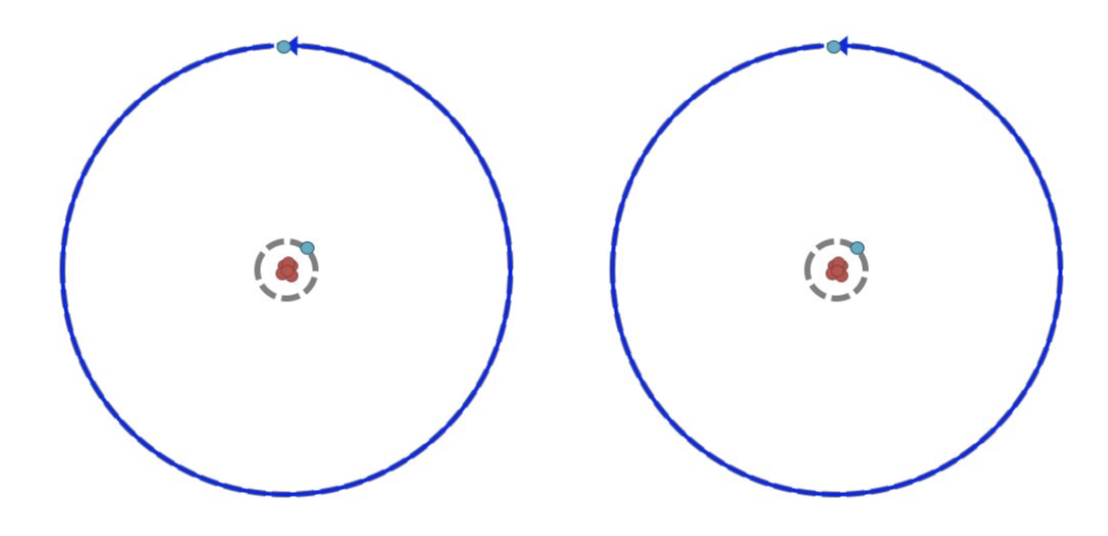
\includegraphics{logos/rydberg_states.png}
      \caption{Another figure caption.}
    \end{figure}








  \end{block}





\end{column}

\separatorcolumn

\begin{column}{\colwidth}

  \begin{block}{Analytic Cases: $V \approx 0, |V| \gg |\Omega|$}

    \begin{itemize}
      \item \textbf{$V \approx 0$.}
      \item \textbf{$|V| \gg |\Omega|$.}
    \end{itemize}




  \end{block}


  \begin{block}{Time Evolution}
    Given the parameters $\Delta, \Omega, \phi_L,$ and $V$ are constant over time, the two-state hamiltonian is time-independent,
    so the propagator is exactly $U(t) = e^{-iH_{int}t/\hbar}$. Given the initial state $|\Psi(0)\rangle$, the joint
    state vector is evaluated at any time $t$ using the following algorithm:
    \begin{enumerate}
      \item \textbf{Rotate}. Find the eigenvectors and eigenvalues of $H_{int}$ and rotate $|\Psi(0)\rangle$ into this eigenbasis
        with a rotation matrix $R$ composed of the eigenvectors.
      \item \textbf{Evolve}. Multiply each of the state's components in the eigenbasis by the propagator $e^{-iE_jt/\hbar}$
      where $E_j$ are the corresponding eigenvalues.
      \item \textbf{Rotate back}. Use $R^\dag$ to rotate the evolved state back into the original basis.
    \end{enumerate}
    Mathematically,
    $$
    |\Psi(t)\rangle = R^\dag D R|\Psi(0)\rangle,
    $$
    where $D$ is the $4x4$ matrix with $e^{-iE_jt/\hbar}$ on the diagonals and zero elsewhere. The time evolution of the initial
    state $|\Psi(0)\rangle=|00\rangle$ was solved for using this method. The probability of remaining in the initial state at
    time $t$, $P_{|00\rangle}=|\langle 00 | \Psi(t) \rangle|^2$, and the probability of transition to the maximally entangled
    bell state $|\Psi^+ \rangle = \frac{1}{\sqrt{2}}(|0r\rangle + |r0\rangle)$,
    $P_{|\Psi^+\rangle}=|\langle \Psi^+ | \Psi(t) \rangle|^2$, were evaluated at each point in time.

  \end{block}



  \begin{block}{Results}

    Nulla eget sem quam. Ut aliquam volutpat nisi vestibulum convallis. Nunc a
    lectus et eros facilisis hendrerit eu non urna. Interdum et malesuada fames
    ac ante \textit{ipsum primis} in faucibus. Etiam sit amet velit eget sem
    euismod tristique. Praesent enim erat, porta vel mattis sed, pharetra sed
    ipsum. Morbi commodo condimentum massa, \textit{tempus venenatis} massa
    hendrerit quis. Maecenas sed porta est. Praesent mollis interdum lectus,
    sit amet sollicitudin risus tincidunt non.

    Etiam sit amet tempus lorem, aliquet condimentum velit. Donec et nibh
    consequat, sagittis ex eget, dictum orci. Etiam quis semper ante. Ut eu
    mauris purus. Proin nec consectetur ligula. Mauris pretium molestie
    ullamcorper. Integer nisi neque, aliquet et odio non, sagittis porta justo.

    \begin{itemize}
      \item \textbf{Sed consequat} id ante vel efficitur. Praesent congue massa
        sed est scelerisque, elementum mollis augue iaculis.
        \begin{itemize}
          \item In sed est finibus, vulputate
            nunc gravida, pulvinar lorem. In maximus nunc dolor, sed auctor eros
            porttitor quis.
          \item Fusce ornare dignissim nisi. Nam sit amet risus vel lacus
            tempor tincidunt eu a arcu.
          \item Donec rhoncus vestibulum erat, quis aliquam leo
            gravida egestas.
        \end{itemize}
      \item \textbf{Sed luctus, elit sit amet} dictum maximus, diam dolor
        faucibus purus, sed lobortis justo erat id turpis.
      \item \textbf{Pellentesque facilisis dolor in leo} bibendum congue.
        Maecenas congue finibus justo, vitae eleifend urna facilisis at.
    \end{itemize}

  \end{block}

\end{column}

\separatorcolumn

\begin{column}{\colwidth}

  \begin{exampleblock}{A highlighted block containing some math}

    A different kind of highlighted block.

    $$
    \int_{-\infty}^{\infty} e^{-x^2}\,dx = \sqrt{\pi}
    $$

    Interdum et malesuada fames $\{1, 4, 9, \ldots\}$ ac ante ipsum primis in
    faucibus. Cras eleifend dolor eu nulla suscipit suscipit. Sed lobortis non
    felis id vulputate.

    \heading{A heading inside a block}

    Praesent consectetur mi $x^2 + y^2$ metus, nec vestibulum justo viverra
    nec. Proin eget nulla pretium, egestas magna aliquam, mollis neque. Vivamus
    dictum $\mathbf{u}^\intercal\mathbf{v}$ sagittis odio, vel porta erat
    congue sed. Maecenas ut dolor quis arcu auctor porttitor.

    \heading{Another heading inside a block}

    Sed augue erat, scelerisque a purus ultricies, placerat porttitor neque.
    Donec $P(y \mid x)$ fermentum consectetur $\nabla_x P(y \mid x)$ sapien
    sagittis egestas. Duis eget leo euismod nunc viverra imperdiet nec id
    justo.

  \end{exampleblock}

  \begin{block}{References}

    Class aptent taciti sociosqu ad litora torquent per conubia nostra, per
    inceptos himenaeos. Phasellus libero enim, gravida sed erat sit amet,
    scelerisque congue diam. Fusce dapibus dui ut augue pulvinar iaculis.

    \begin{table}
      \centering
      \begin{tabular}{l r r c}
        \toprule
        \textbf{First column} & \textbf{Second column} & \textbf{Third column} & \textbf{Fourth} \\
        \midrule
        Foo & 13.37 & 384,394 & $\alpha$ \\
        Bar & 2.17 & 1,392 & $\beta$ \\
        Baz & 3.14 & 83,742 & $\delta$ \\
        Qux & 7.59 & 974 & $\gamma$ \\
        \bottomrule
      \end{tabular}
      \caption{A table caption.}
    \end{table}

    Donec quis posuere ligula. Nunc feugiat elit a mi malesuada consequat. Sed
    imperdiet augue ac nibh aliquet tristique. Aenean eu tortor vulputate,
    eleifend lorem in, dictum urna. Proin auctor ante in augue tincidunt
    tempor. Proin pellentesque vulputate odio, ac gravida nulla posuere
    efficitur. Aenean at velit vel dolor blandit molestie. Mauris laoreet
    commodo quam, non luctus nibh ullamcorper in. Class aptent taciti sociosqu
    ad litora torquent per conubia nostra, per inceptos himenaeos.



  \end{block}

  \begin{block}{References}

    \nocite{*}
    \footnotesize{\bibliographystyle{plain}\bibliography{poster}}

  \end{block}

\end{column}

\separatorcolumn
\end{columns}
\end{frame}

\end{document}
